\section{Numerical example}

Let us consider the Lorenz system, $i.e.$,
\begin{align}
	\dv{x}{t} &= \sigma(y - x), \\
	\dv{y}{t} &= x(\rho - z) - y, \\
	\dv{z}{t} &= xy - \beta z,
\end{align}
where $\sigma = 10, \rho = 28, \beta = 8/3$. We provide the system with initial conditions
\begin{equation}
	x(0) = -10, \quad y(0) = -1, \quad z(0) = 40, 
\end{equation}
and integrate the system up to the final time $T = 20$. We choose as deterministic integrator the classic fourth-order Runge-Kutta method, with timestep $h = 0.001$. Results show that the realizations of the numerical solutions obtained with the probabilistic method follow the behaviour of the deterministic method in the first part of the time span and then show a chaotic behaviour, revealing the features of the underlying system. The three components $x, y, z$ of the solution obtained with the deterministic and probabilistic solvers are depicted in Figure \ref{fig:Lorenz}. 

\begin{figure}[t]
	\centering
	\begin{subfigure}{1\linewidth}
		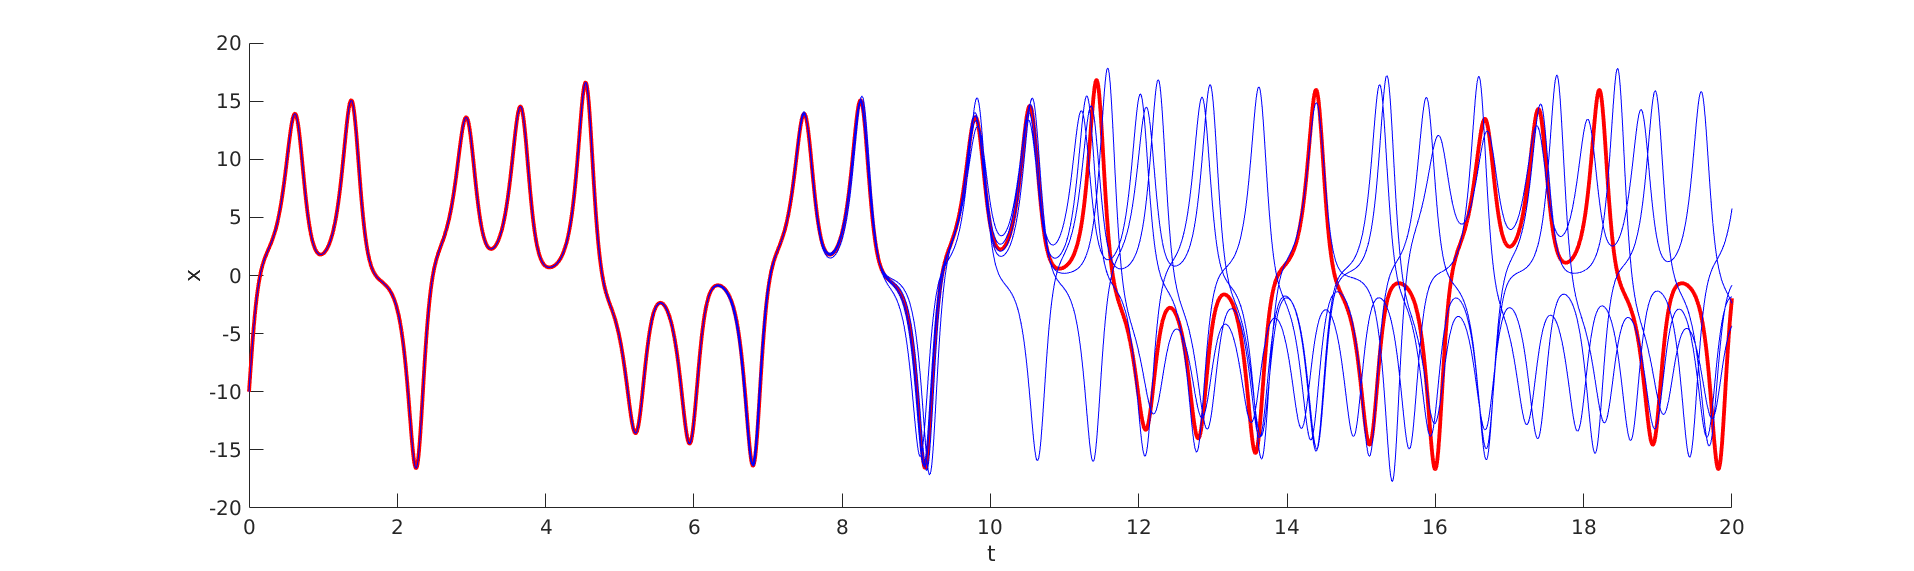
\includegraphics[width=1\linewidth]{plots/Lorenz_x.png}
	\end{subfigure}
	\begin{subfigure}{1\linewidth}
		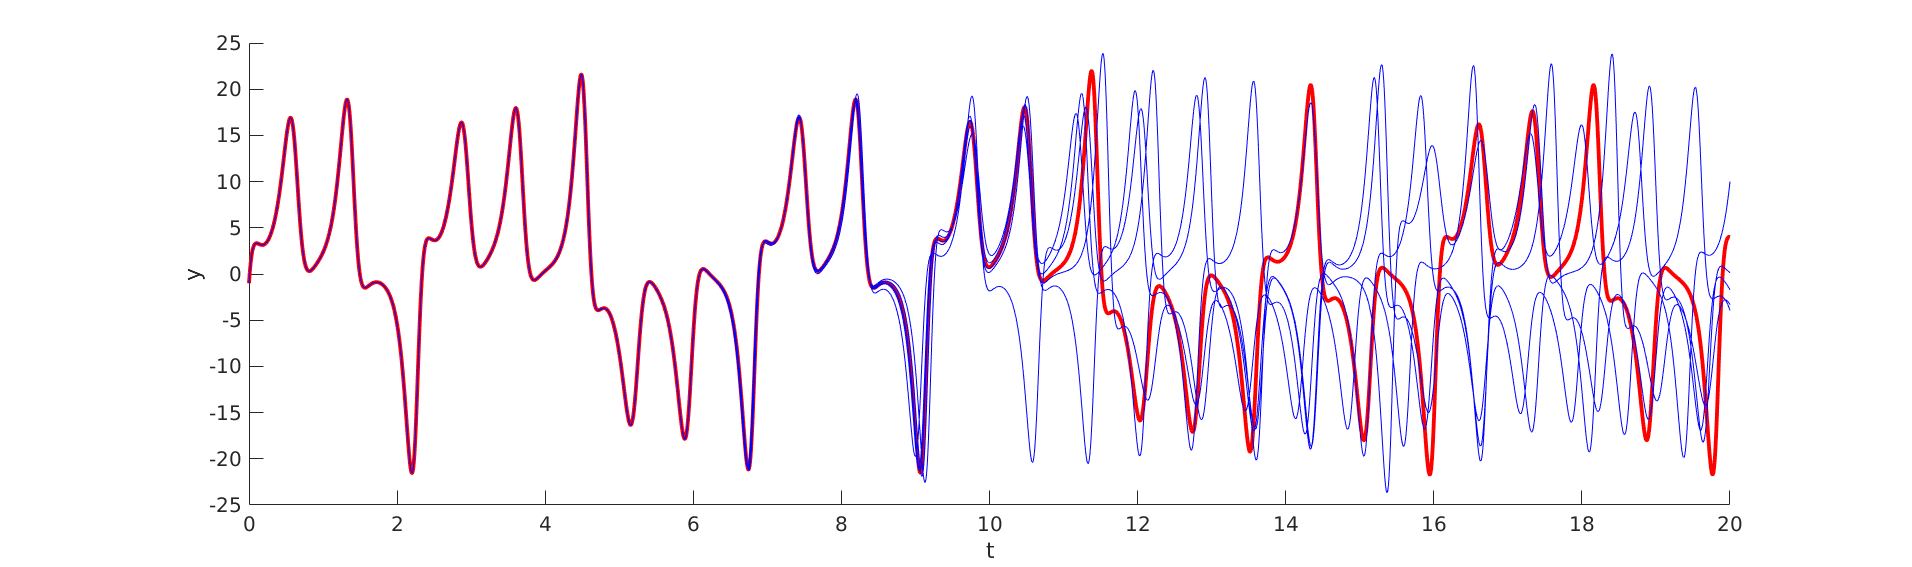
\includegraphics[width=1\linewidth]{plots/Lorenz_y.png}
	\end{subfigure}
	\begin{subfigure}{1\linewidth}
		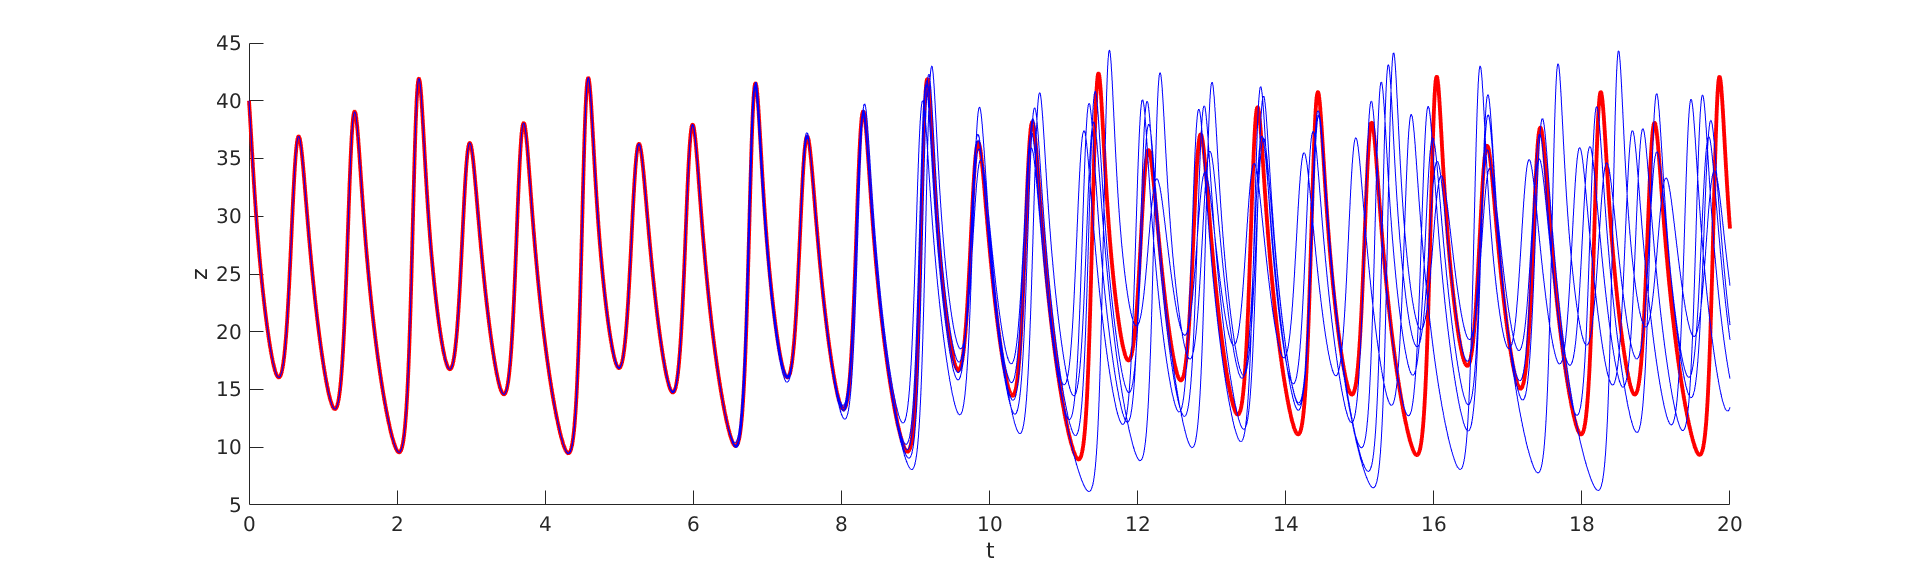
\includegraphics[width=1\linewidth]{plots/Lorenz_z.png}
	\end{subfigure}
	\caption{Solution of the Lorenz system obtained with the deterministic solver (red) and realizations of the solution obtained with the probabilistic solver (blue).}
	\label{fig:Lorenz}
\end{figure}
